% !TEX root = ../my-thesis.tex
%
\chapter{Review}
\label{sec:review}

\section{Stochastic Computing: Fundamental Concepts}
\label{sec:review:sec1}

Stochastic Computing (SC) circuits represent a paradigm shift in computational method, enabling arithmetic functions with minimal logic gates. This is achieved by  encoding values into patterns of random bit sequences, a stochastic number. For example, the number $\frac{1}{3}$ can be shown as a series of bits like $0, 0, 1, 0, 1, 0$, where the number of 1's is one-third of the total.

In this framework, each bit in the series is considered a random variable, $X$, following a Bernoulli distribution with a probability $p_X$ of being 1. $X$ is also used to denote the stochastic number that is collectively represented by a series of bits, commonly referred to as bit sequences or bitstreams. As big letters i.e $X$ denote stochastic numbers, $p_X$ denote probabilities encoded in the bitstreams, we use small letters i.e $x$ for the actual values linked to stochastic numbers.

There are two major ways to represent actual values as stochastic number. For a positive real parameter $M$, the unipolar stochastic number $X$ could represent a non-negative real number $x$ such that $0 \leq x \leq M$ by having $p_X = \frac{x}{M} $. On the other hand, the bipolar stochastic number $X$ could represent a real number $x$ such that $-M \leq x \leq M$ by having $p_X  = \frac{x}{2M} + \frac{1}{2}$.

We could also interpret that in unipolar encoding, zeros in the bitstream are weighted as 0 and ones are weighted as +1, thus limits unipolar encoding to the positive range [0, M]. On the other hand, bipolar encoding weights zeros as -1 and ones as +1, allowing the range [-M, +M]. Thus depend on the format, we would configure the counter circuit of Stochastic-to-Digital Converters (SDC) differently to return the correct value in binary format. 


\textbf {Correlation}

The correlation between bitstream is a major consideration when designing SC circuit. Most SC circuits operate best with a specific input SN correlation. The correlation level between bitstreams is assessed using the stochastic computing correlation (SCC). An SCC value of +1.0 signifies maximum positive correlation, -1.0 indicates maximum negative correlation, and 0.0 implies the bitstreams are uncorrelated. 

For example, the circuit for multiplying with AND Gate for unipolar encoding or XOR Gate for bipolar encoding works best with uncorrelated bitstream. Accuracy in computation improves as the correlation of input bitstreams approaches the optimal SCC value.

By contrast, some operations would be possible with positive correlation, while for some it would not be necessary to take correlation into consideration. 


\section{Stochastic Computing Elements}
\label{sec:review:sec3}

In stochastic computing, some computational elements can be effectively implemented using fundamental gates with minimal footprint. This stems from the observation that NOT Gates  the complement of input event AND Gates joint probability OR Gates the union of two independent events:

$\bullet$ NOT Gate: $p_Q = 1 - p_X$ \\
$\bullet$ AND Gate: $p_Q = p_X p_Y$ \\
$\bullet$ OR Gate: $p_Q = p_X + p_Y - p_Xp_Y$ \\

Therefore, multiplication could be conducted using a singular AND gate in the case of unipolar encoding or a singular XNOR gate in the case of bipolar encoding. 

Letting two bitstreams represent stochastic numbers A and B pass through an AND gate, the resulting SN Q encodes the probability of $p_Q = p_X p_Y$. With unipolar mappings applied, and suppose the output scale constant $M_Q = M_X M_Y$ whereas $M_X, M_Y$ are input scale constants, we have: $$p_Q = \frac{x}{M_X}\frac{y}{M_Y} = \frac{xy}{M_Q}  \rightarrow  \frac{q}{M_Q}$$

Similarly, letting the inputs through an XNOR gate, the resulting SN Q encodes the probability of $p_Q = 1 - p_X (1-p_Y) - (1-p_X) p_Y = 1 - p_X - p_Y = 1 - \frac{x}{M_X} - \frac{y}{M_Y}$ 

inputs \(a\) and \(b\), and output \(q\), the relationship is established as \(q + \frac{1}{2} = -(a + \frac{1}{2} + b + \frac{1}{2} - (a + 1) \times (b + 1) / 2)\). Simplifying this equation yields \(q = a \times b\), thus interpreting the XNOR gate as a multiplier in the bipolar context.

Multiplcation with a singular gate is one of the major reason SC economic compare to conventional circuit. However, the bitstream into multiplication must be uncorrelated i.e independent for accuracy. 

In addition to multiplication, scaled addition could be effectly implement with combinational stochastic computing using a multiplexer (MUX) for both bipolar and unipolar formats. The select input of the MUX, \(S\), is always a unipolar stochastic number with $M = 1$ as it functions as a weighting factor ranging from 0 to 1. Thus $$p_Q = (1 - p_S) \times p_X + p_S \times p_B$$; setting $p_S = 0.5$ effectively averaging the probabilities of the two inputs.

Scaled subtraction is exclusive to the bipolar format and is achieved through a combination of a MUX and a NOT gate. In contrast, the inverse operation in unipolar coding is straightforwardly implemented using a NOT gate. 

We also note that for MUX operation, only the correlation between select signal and inputs affect the correctness of output while the correleation between inputs have no impact.  

In addition to operation on independent 
The maximum (max) and minimum (min) value functions are two useful functions
with simple and low cost unary implementation. In a weighted binary design,
data-width-dependent comparator and multiplexer units must be used to implement
these functions. In unary processing, individual gates can synthesize these
functions: an AND gate gives the minimum of two unary streams when two
equal-length unary streams are connected to its inputs; an OR gate gives the
maximum value when its inputs are fed with two equal-length unary streams.
Absolute-valued subtraction: XOR gate



However, combinational logic alone could not realize all functions i.e computing the absolute value or performing arithmetic comparisons poses a challenge. This is where stochastic computational elements based on sequential logic, like Finite State Machines (FSMs), come into play. FSMs extend the capabilities of SC, enabling the execution of more complex functions that combinational logic struggles with. By integrating sequential logic, SC broadens its application scope, catering to a wider range of computational needs while maintaining its inherent simplicity and efficiency.

\begin{figure}[htb]
	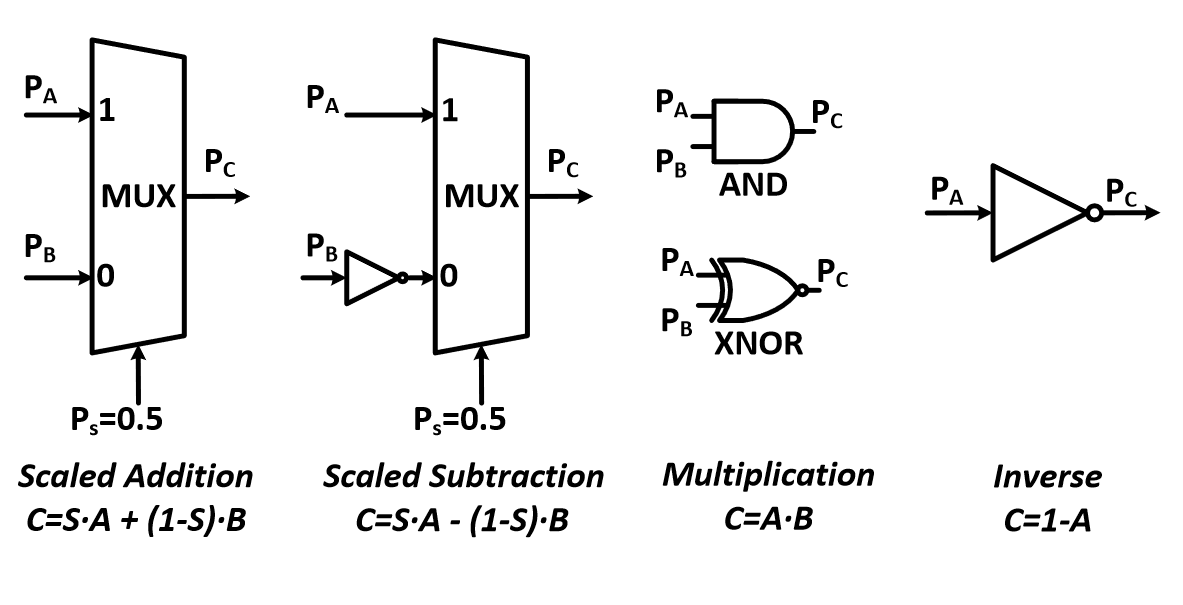
\includegraphics[width=10cm]{gfx/SC elements.png}
	\caption{Stochastic computational elements}
	\label{fig:system:example1}
\end{figure}

\begin{figure}[htb]
	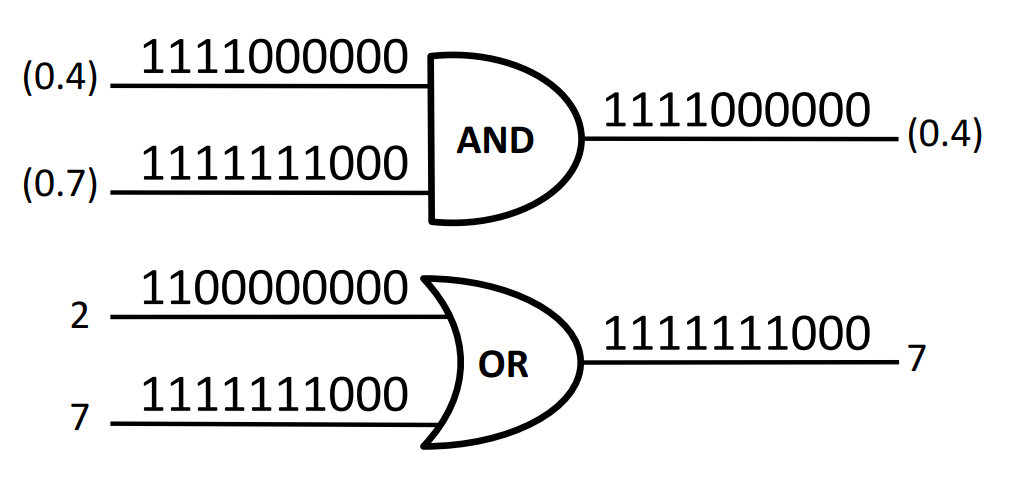
\includegraphics[width=10cm]{gfx/maxmin.png}
	\caption{Computational elements with correlated bitstream}
	\label{fig:system:example1}
\end{figure}




Conventional approach of generating stochastic signals is costly!
– Expensive SNGs
– High latency, High energy consumption
• Proposed a low-cost energy-efficient approach for generating
stochastic signals based on PWM signals
– Area, latency, energy consumption are all greatly reduced
– 99% performance speedup,
– 98% saving in energy dissipation,
– and 40% area reduction compared to prior stochastic approaches
• The proposed mixed-signal approach
– Inherits the fault-tolerant advantage of stochastic design
– Working as fast and energy efficiently as conventional binary designs

\section{Bitstream Representations of Values}
\label{sec:review:sec2}

The accuracy of a stochastic number gets better with a longer sequence, a
feature called progressive precision. At least 11 bits are needed to encode the
probability $5/11$; at least 16 bits are needed to encode $5/16$. Since the
bits are random, you often need a much longer sequence to get close to the exact
average you want. However, in real-life, stochastic numbers often aren't perfect
because the bits can be influenced by previous bits in the sequence. This can
make the computations less efficient or accurate There are two types of
stochastic numbers: `ideal,' where each bit is independent and doesn't rely on
the previous bits, and `non-ideal,' where the bits are influenced by their
history in the sequence.



\subsection{Bitstream Generation}

\textbf {Linear-Feedback Shift Registers}

A popular method for generating random numbers in stochastic computing (SC) is
using a linear-feedback shift register (LFSR). An N-bit LFSR consists of N
flip-flops and XOR gates, forming a feedback loop. With N bits, there are
$ (2^ N - 1)$ potential combinations leaving zero. As a maximal LFSR
cycles through these  $(2 N - 1 )$ numbers in a pseudo-random order, it can generate approximately  $2^ {n-1}$ bits long stochastic bitstream. 

To ensure multiple bitstreams remaining uncorelated, LFSRs may be configured with different seeds. Each LFSR would go through the same sequence but at different stages. 

To alleviate the cost of LFSRs, a sharing scheme may be applied by utilizing memory component like flipflop to vary the stage of the same LFSRs. 


\textbf {Low-Discrepancy Sequences}

Low Discrepancy (LD) sequences, such as the van der Corput/Halton sequence and
the Sobol' sequence, are used in stochastic bitstream generation for their
equidistribution properties. These sequences distribute more evenly compared to
pseudo-random sequences generated by LFSRs, leading to faster convergence in
probability calculations. The van der Corput sequence, a one-dimensional LD
sequence, is created by reversing the digits of natural numbers in a specific
base. The Halton sequence extends this to higher dimensions using co-prime bases.
The Sobol' sequence, a base-2 sequence, is also notable for its distinct,
infinite-length properties.


\subsection{Deterministic Bitstream}

Our approach is motivated by the following observation: a stochastic representation is a uniform, fractional representation. All that matters in terms of the value that is computed is 
the fraction of the time the signal is high

Stochastic Operations with Correlated Inputs:
– Correlation in PWM signals:
• Choosing the same frequency for the input signals
• Having maximum overlap between the high parts
– We call two correlated PWM signals:
Synchronized PWM signals
– Advantage: Accurate output after running for only one period
– Eliminating random fluctuation inaccuracy
– Limitation: Difficult to provide synchronization (correlation) in the
second (or higher) levels of the circuit.



\begin{figure}[htb]
	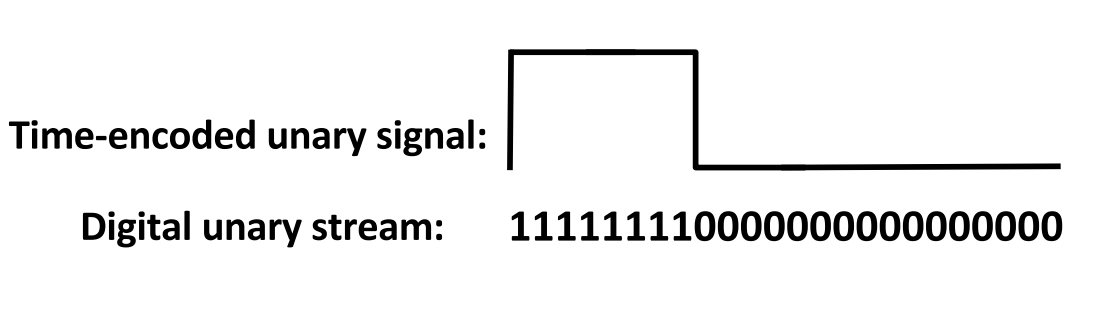
\includegraphics[width=10cm]{gfx/Time-encode signal.png}
	\caption{Time-based bitstream}
	\label{fig:system:example1}
\end{figure}

\subsection{Dynamic Bitstream}

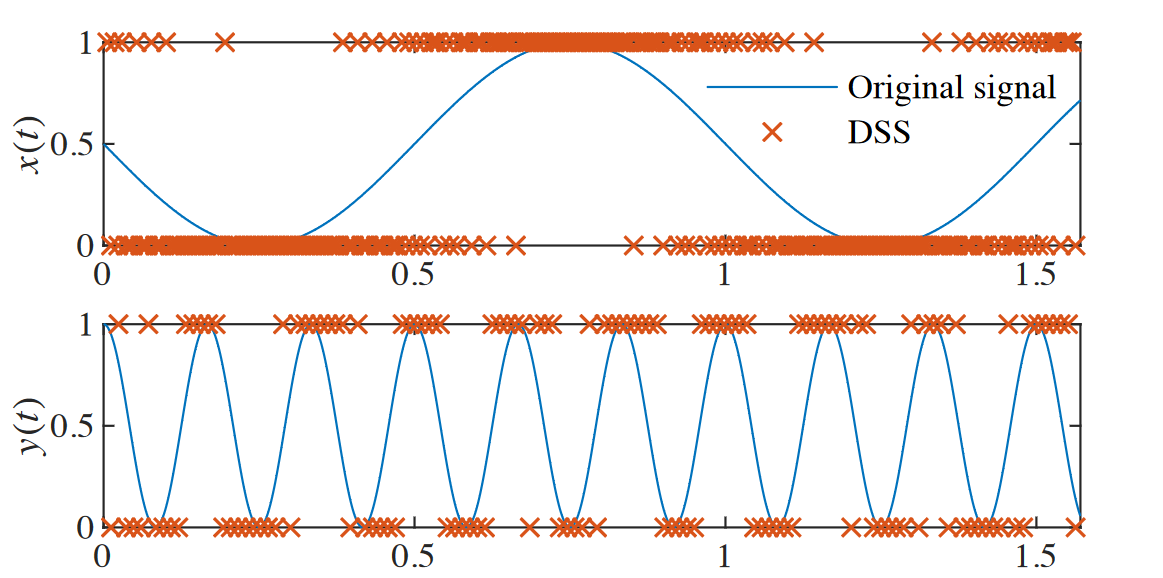
\includegraphics[width=10cm]{gfx/DSC.png} 

\begin{figure}[htb]
	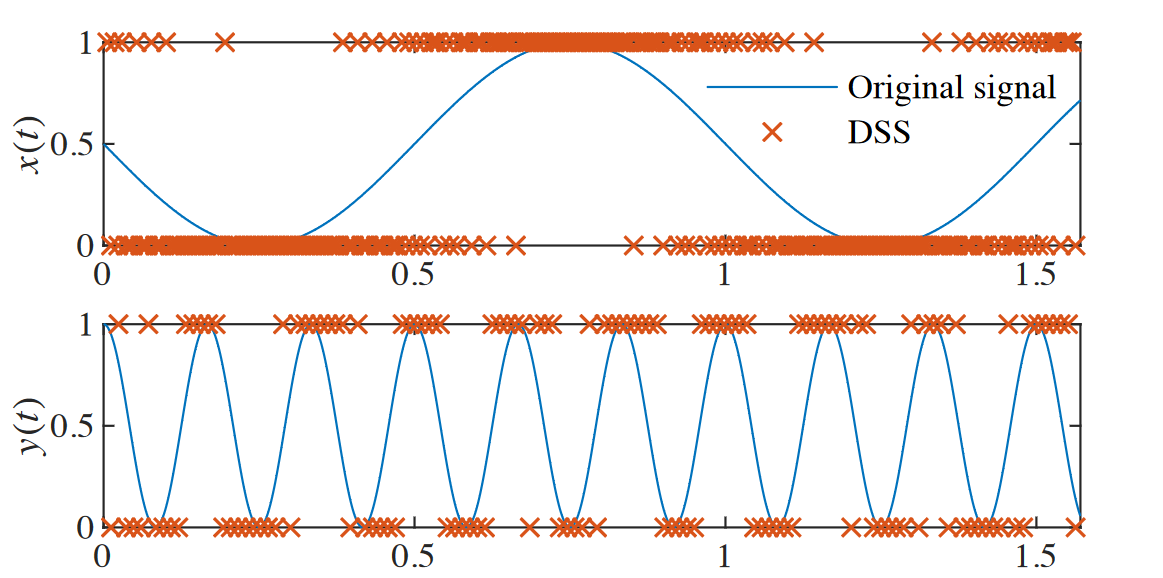
\includegraphics[width=10cm]{gfx/DSC.png} 
	\caption{Example of dynamic stochastic bitstream}
	\label{fig:system:example2}
\end{figure}


Addressing and reducing the effect of unwanted SN correlation is a significant challenge in SC design. There are three main strategies for controlling correlation: (1) employing circuits insensitive to correlation, (2) using circuits that manipulate correlation, and (3) carefully choosing number sequences for Stochastic Number Generators (SNGs). The first strategy involves using special circuit designs that are less affected by correlation levels, although they may require more power and space, and aren't available for all SC arithmetic operations. The second method includes implementing circuits that can alter the correlation of existing SNs, such as isolators, synchronizers, desynchronizers, decorrelators, and regenerators. The third method is the careful selection of number sequences for SNGs. Research has shown that low discrepancy sequences like Van der Corput, Halton, and Sobol are preferable due to their favorable correlation properties. Other useful sequences include Linear Feedback Shift Registers (LFSRs), ramp sequences, and unconventional SNGs like pulse-width modulated signals, rotated bitstreams, and pre-generated bitstreams. Designing deterministic number sequences for SC circuits remains a complex task with limited general methods.

For combinational SC circuits, it's also possible to rotate or swap number positions within each sequence without affecting computation accuracy, as long as the relative ordering of numbers is maintained. This concept, known as relative ordering invariance, ensures that the correlation between number sequences is preserved. However, this principle doesn’t apply to sequential circuits, which are sensitive to autocorrelation that is not maintained under these transformations.

In addition, Qian et al [13] proposed a synthesis approach based on MUX and Full-Adder to take advantage of Bernstein polynomial in stochastic computing. This technique can be used to approximate both linear and nonlinear polynomials. However, it works only for the unipolar format. Any function that can be represented using the above operations can be implemented stochastically with very simple combinational circuits. However, there are many functions which do not meet this requirement, such as computing absolute value and making an arithmetic comparison, and so cannot be easily implemented with these combinational logic gates. Fortunately, stochastic computational elements based on FSM can resolve this issue


\section{Function Approximations}
\label{sec:review:sec4}


